\section{Predecessors}

\subsection{VLab}

\begin{frame}{VLab}
    \begin{columns}[t]
        \begin{column}[T, onlytextwidth]{0.4\textwidth} % See https://tex.stackexchange.com/a/351465/61591
            \begin{itemize}
                \item The Virtual Laboratory for Earth and Planetary Materials
                      (VLab)\footnotemark, was
                      funded by the NSF in 2004 at the Minnesota Supercomputing Institute.
                \item VLab is a cyberinfrastructure consisting a fully integrated web
                      portal, web services, and databases for ab initio calculations of
                      planetary materials.
            \end{itemize}
        \end{column}

        \begin{column}[T]{0.6\textwidth}
            \begin{tikzpicture}[baseline=(current bounding box.north)]
                \node (a) {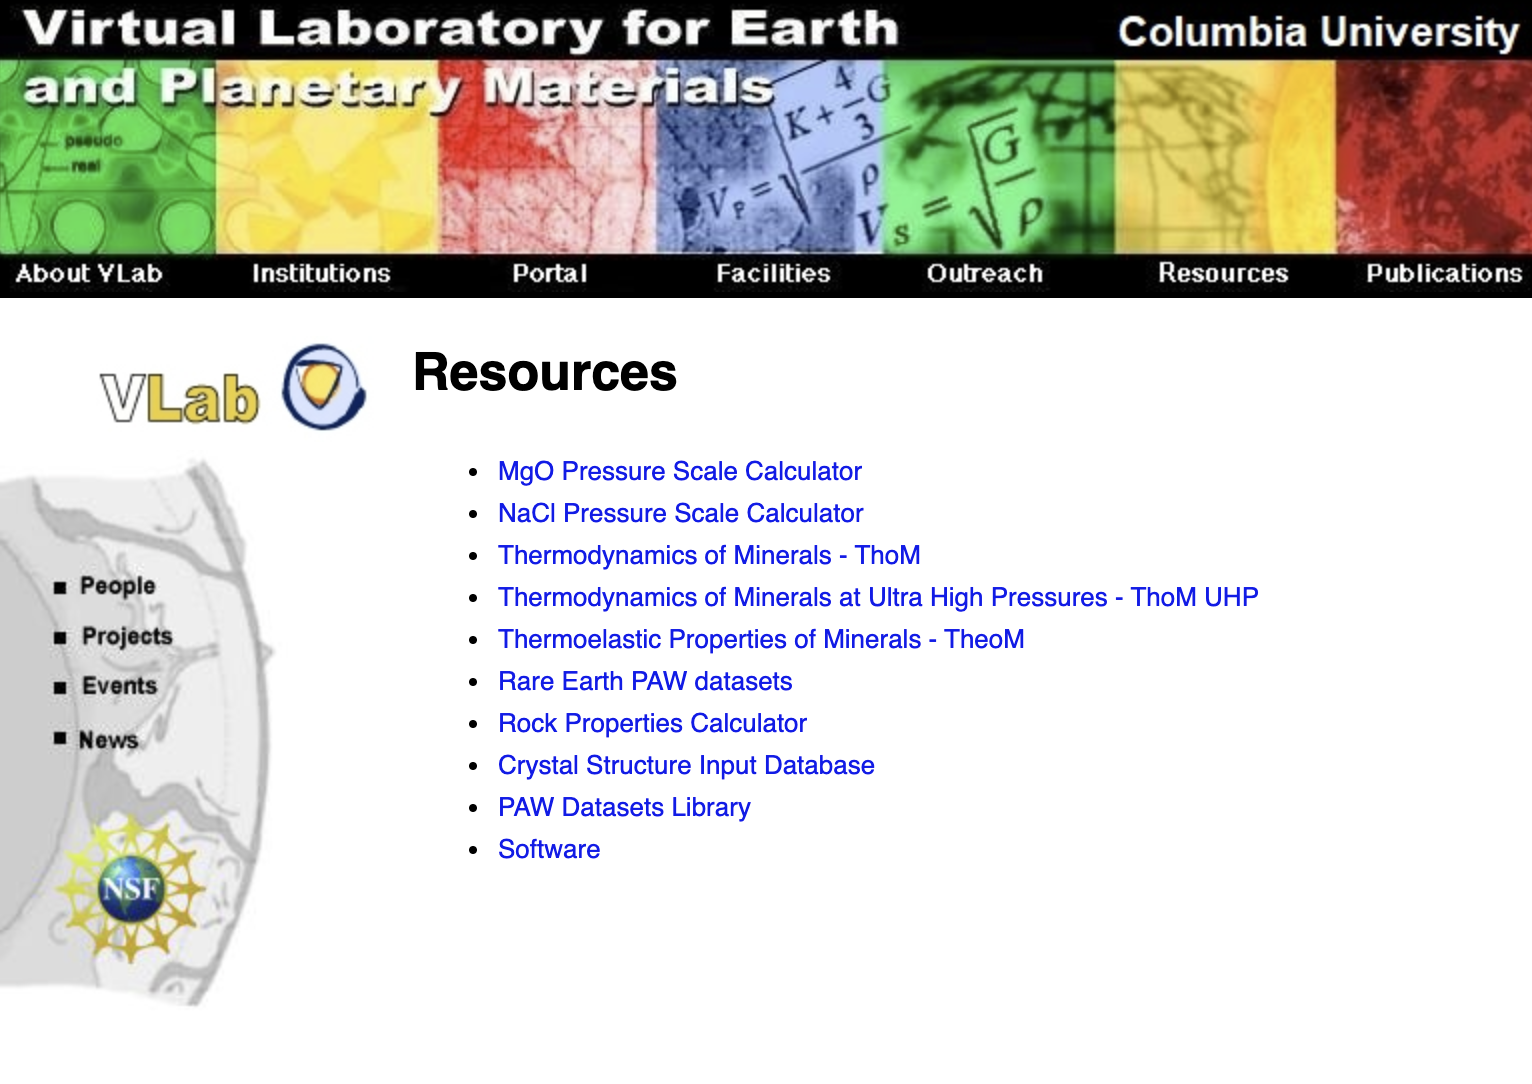
\includegraphics[width=\textwidth]{vlab}};
                \node [below=-0.5cm of a] {\url{http://mineralscloud.com/resources/}};
            \end{tikzpicture}
        \end{column}
    \end{columns}
    \footcitetext{DASILVA2007321}

    \begin{tikzpicture}[overlay, remember picture]
        \node[xshift=-0.9cm,yshift=-0.9cm] at (current page.north east) {\qrcode[height=1.8cm]{http://mineralscloud.com/resources/}};
    \end{tikzpicture}
\end{frame}

\subsection{\texttt{qha}}

\begin{frame}{\texttt{qha}: quasiharmonic free energy calculation for multi-configuration systems}
    \begin{columns}[t]
        \begin{column}[T, onlytextwidth]{0.4\textwidth} % See https://tex.stackexchange.com/a/351465/61591
            We drew inspiration from our published and unpublished code, e.g.
            \texttt{qha}\footnotemark, when developing the current workflows.

            For example, \texttt{qha} runs with a human-readable
            configuration file and a given input.
            The same mechanism is adopted in \express{}.
            See subsection \ref{ssec:ui}.
        \end{column}

        \begin{column}[T]{0.6\textwidth}
            \begin{tikzpicture}[baseline=(current bounding box.north)]
                \node (a) {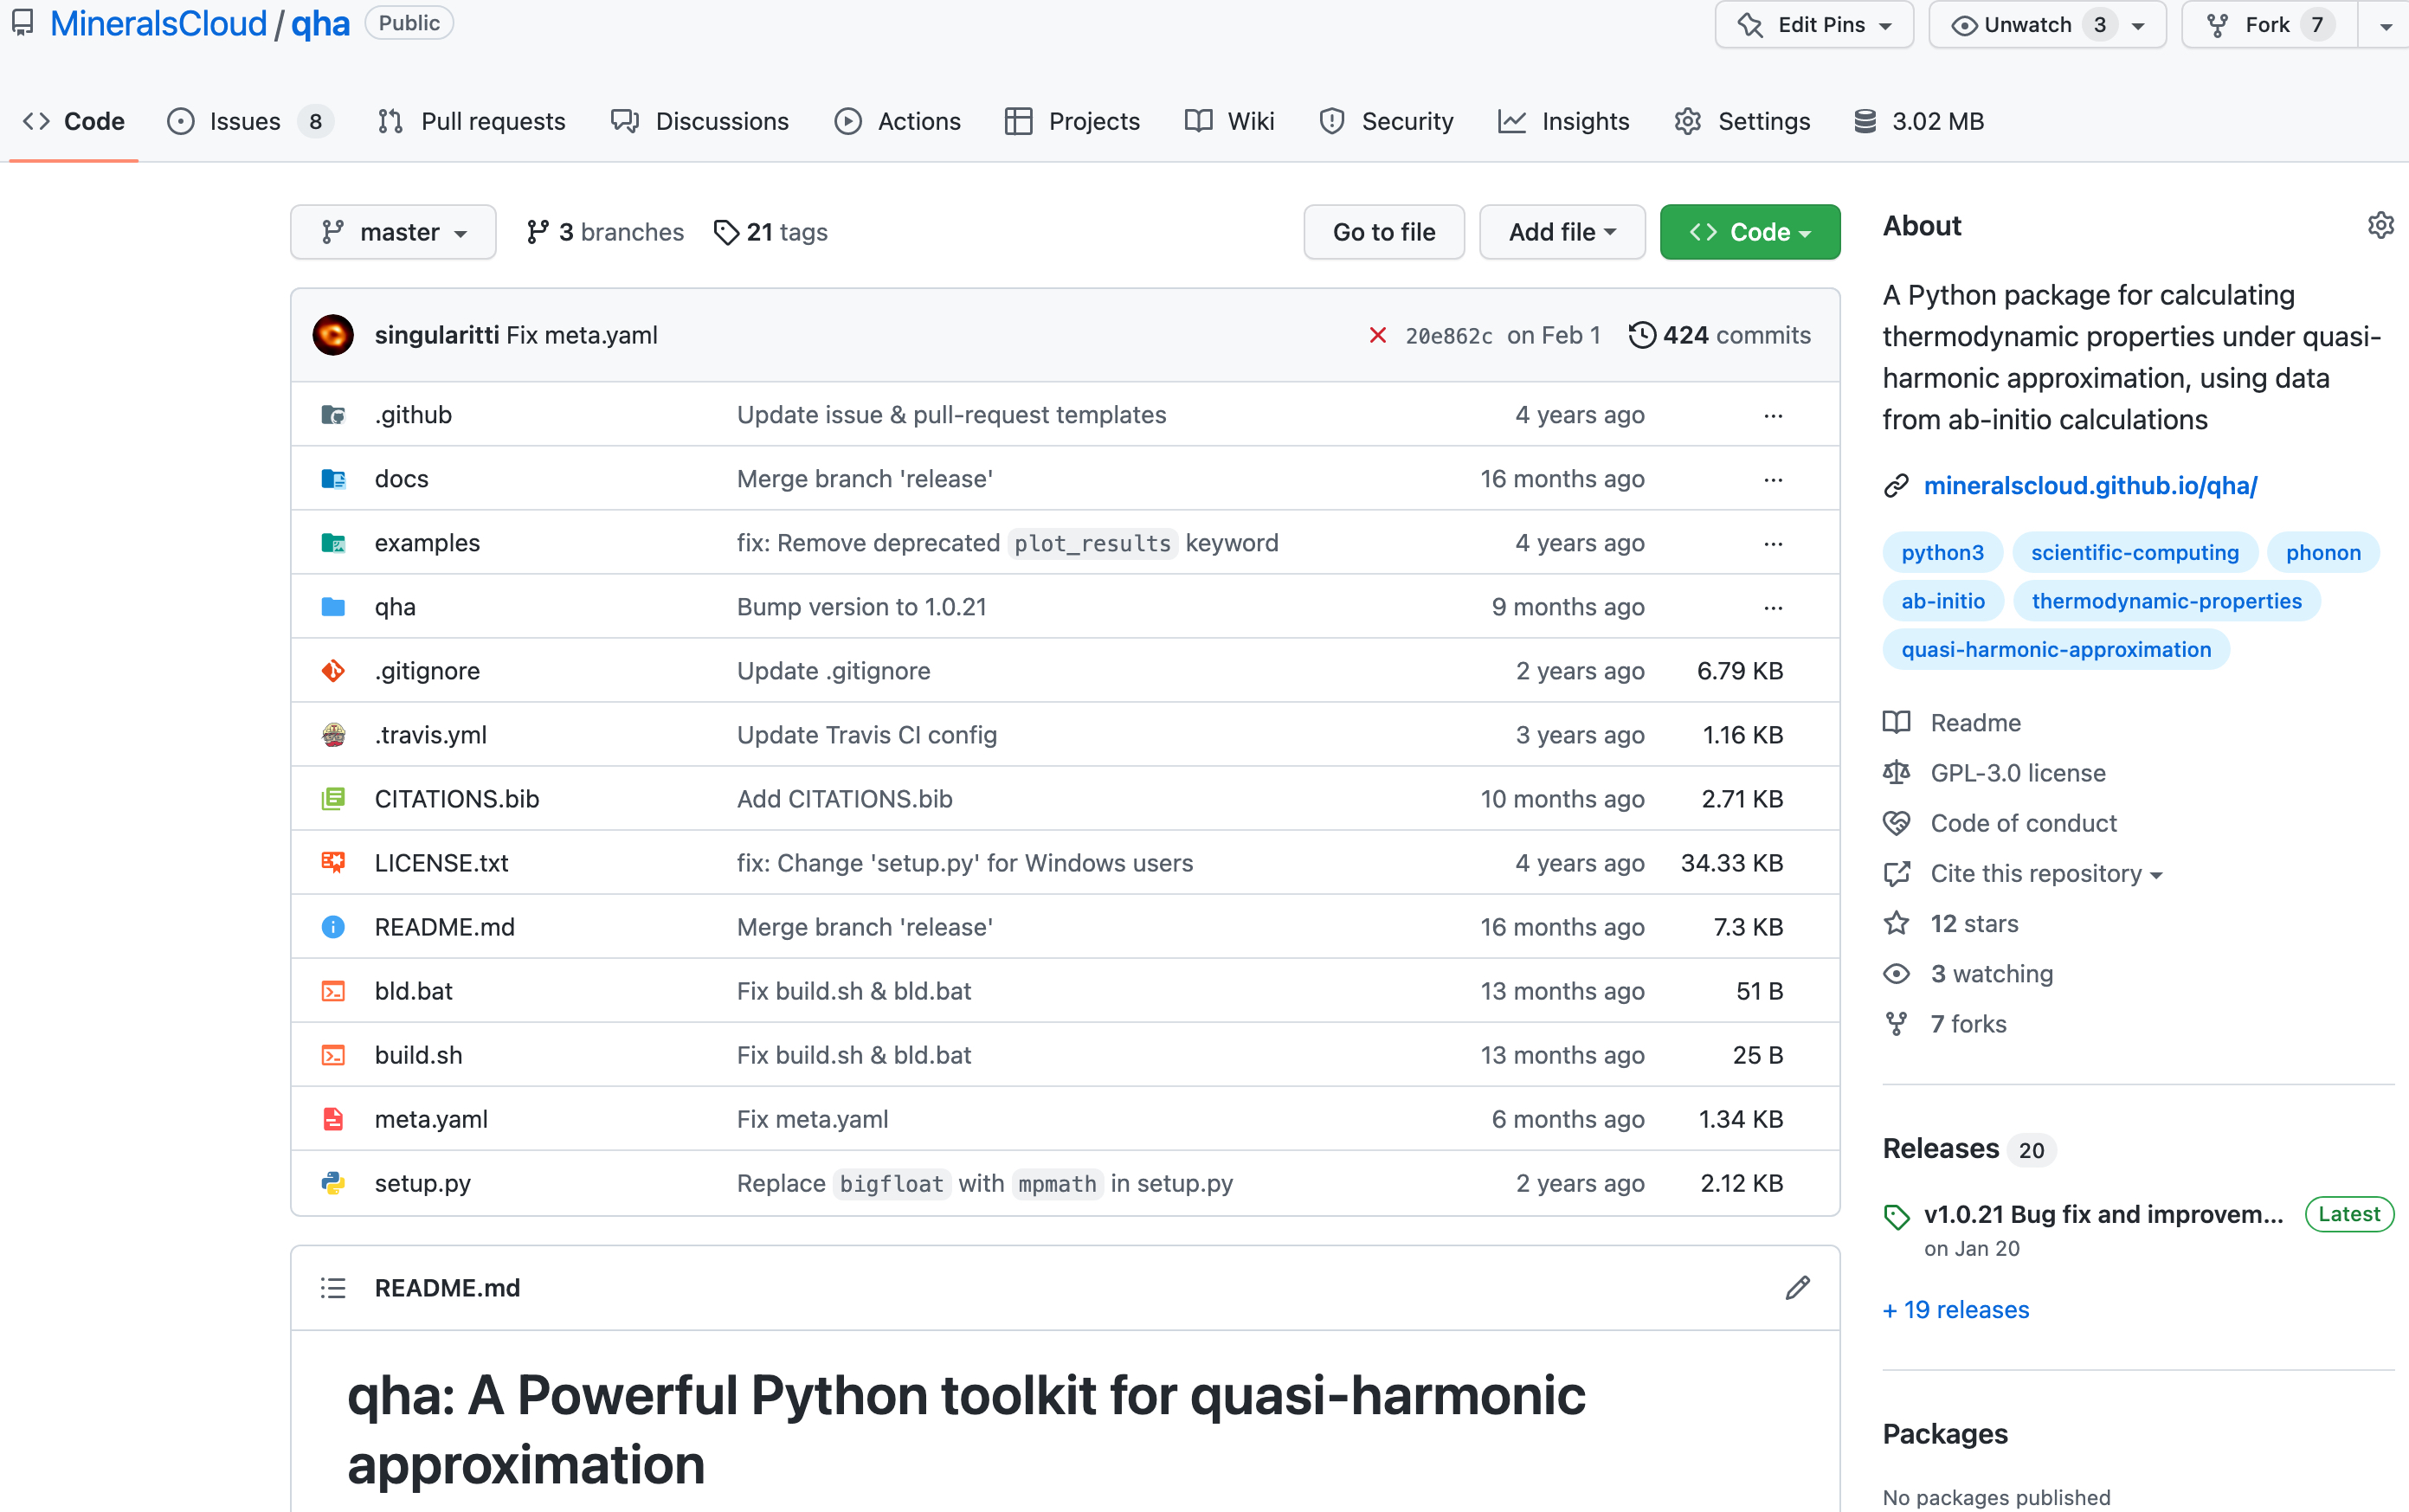
\includegraphics[width=\textwidth]{qha}};
                \node [below=0cm of a] {\url{https://github.com/MineralsCloud/qha}};
            \end{tikzpicture}
        \end{column}
    \end{columns}
    \footcitetext{QIN2019199}

    \begin{tikzpicture}[overlay, remember picture]
        \node[xshift=2cm,yshift=2cm] at (current page.south west) {\qrcode[height=2cm]{https://github.com/MineralsCloud/qha}};
    \end{tikzpicture}
\end{frame}
